\documentclass[a4paper, 12pt]{book}

\usepackage[T1]{fontenc}
\usepackage[utf8]{inputenc}
\usepackage[italian]{babel}
\usepackage{quoting}
\usepackage{graphicx} %per inserire immagini nel testo
\usepackage{sidecap} %permette di aggiungere didascalie alle immagini
\usepackage{subfig}
\usepackage[colorlinks]{hyperref} %per rendere interattivo il documento, gli elementi interattivi saranno in rosso con l'opzione colorlinks
\usepackage{amsmath}
\usepackage{amsthm} %per enunciati
\usepackage{bohr}
\theoremstyle{plain}
\newtheorem{teorema}{Teorema}[section]
\usepackage{geometry}
\geometry{a4paper, top = 3cm, bottom = 3cm, left = 3.5cm, right = 3.5cm, heightrounded, bindingoffset = 5mm}
\pagestyle{plain}

\author{Giovanni Tosini}
\title{Fisica II}
\date{ }

\begin{document}
\begin{titlepage}
    \maketitle
\end{titlepage}

\frontmatter %numeri romani prima del testo effettivo
\tableofcontents
\mainmatter %numeri arabi dalla prima pagina di testo effettivo

\chapter{Introduzione}

Esistono due tipi di forze in assoluto:
\begin{itemize}
    \item  attrattive
    \item repulsive
\end{itemize}
Queste forze si possono vedere anche nelle singole cariche elettriche, quelle con identica carica
si respingeranno, mentre quelle con carica opposta si attrarranno.

Esistono tre modalità per caricare un oggetto:
\begin{itemize}
    \item strofinio
    \item induzione
    \item contatto
\end{itemize}
Da notare che la carica non dipende dal meccanismo con cui viene creata, ma dai costituenti
della materia.
\begin{center}
    \textbf{\textbf{\bohr{10}{A}
    \setbohr{nucleus-radius=1.5em}}}    
\end{center}
Un atomo è composto da: protoni, neutroni ed elettroni. La differenza di dimensioni tra un protone
e un elettrone è di parecchi ordini di grandezza. La carica elettrica di un elettrone viene 
denominata "carica elementare", è tale perché si dice "quantizzata" essendo che si possono trovare solo
cariche multiple di essa. Inoltre il modulo della carica di un elettrone è equivalente alla carica di
 un protone, sebbene siano due particelle differenti.
 \begin{quote}
     \begin{math}
         |qe^-| = qe^+
     \end{math}
 \end{quote}
 La materia ordinaria è neutra, di conseguenza pure l'atomo è neutro, ovvero il centro di 
 simmetria del nucleo coincide con quello degli elettroni.

 Con lo strofinio vengono strappati gli elettroni meccanicamente, nel sistema isolato d'esempio
 (in un sistema isolato la carica totale Q si conserva) preso in questione. La carica dipenderà 
 dal potenziale di estrazione del materiale.

 Per induzione invece, un oggetto \begin{math}
     q^+
 \end{math} avvicinato a un oggetto neutro, porterà a una divisione di cariche nell'oggetto neutro 
 causato dall'induzione elettrostatica
 \begin{center}
     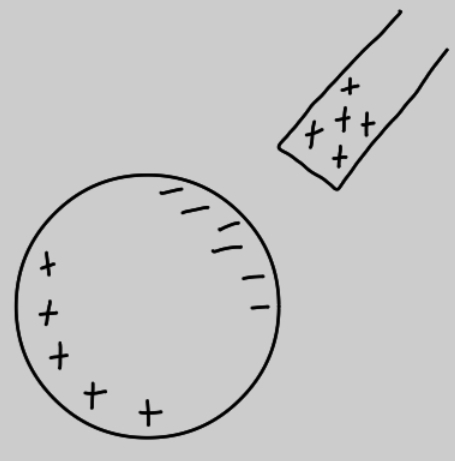
\includegraphics[width=0.5\textwidth]{induzione_elettrostatica.jpg}
 \end{center}

 \chapter{Elettrostatica nel vuoto (in assenza di materia dielettrica)}

Quando non c'è dipendenza dal tempo il campo elettrico e il campo magnetico sono separati.

\section{Interazione (forze) di Coulomb}

\begin{center}
    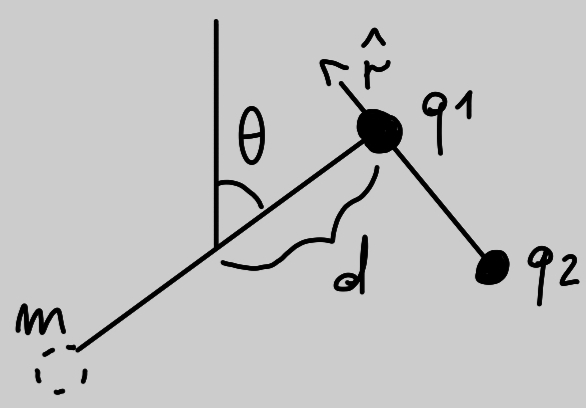
\includegraphics[width=0.5\textwidth]{coulomb.jpg}
\end{center}

\begin{itemize}
    \item m oggetto di massa m, trascurabile
    \item \begin{math}
        \theta
    \end{math} angolo
    \item $q_1$ e $q_2$ sono le cariche
    \item d la distanza
    \item r il versore
\end{itemize}

La forza esercitata lungo d sarà equivalente a:
\begin{quote}
    \begin{math}
        |\vec{F}|=k\frac{q_1q_2}{r^2}
    \end{math}
\end{quote}
Questo è un modello valido \textbf{esclusivamente} per cariche ferme nel vuoto. La costante k 
equivale a
\begin{quote}
    \begin{math}
        k=\frac{1}{4\pi\epsilon_0}
    \end{math}
\end{quote}
Di conseguenza la forza esercitata su $q_1$ sarà equivalente a
\begin{quote}
    \begin{math}
        \vec{F}=\frac{1}{4\pi\epsilon_0}\frac{q_1q_2}{r^{2}_{1,2}}
    \end{math}
\end{quote}

N.B.: \begin{itemize}
    \item l'unità di misura della carica equivale al Coulomb, q = [C].
    \item \begin{math}
        \epsilon_0
    \end{math} è la permeabilità sul vuoto (  costante dielettrica del vuoto)
    \item \begin{math}
        r_{1,2} = \vec{r}_{12} = \vec{r}_2 - \vec{r}_1
    \end{math}
    \item se \begin{math}
        q_1q_2
    \end{math} è positivo allora avremo a che fare con una forza repulsiva, se negativo attrattiva
\end{itemize}

\begin{center}
    \includegraphics*[width=0.5\textwidth]{coulomb_2.png}
\end{center}
\begin{center}
    \includegraphics*[width=0.5\textwidth]{coulomb_3.png}
\end{center}
Una carica $q_0$ in uno spazio vuoto, con attorno N cariche, sarà sotto l'effetto della somma della forza di tutte:
\begin{quote}
    \begin{math}
        \sum_{i = 1}^N \frac{q_iq_0}{4\pi\epsilon_0}\frac{\hat{r}_{i0}}{r_{{i0}^2}}
    \end{math}
\end{quote}
N.B.: \begin{itemize}
    \item l'unità di misura della forza è il Newton [N]
    \item \begin{math}
        \hat{r_{12}} = \hat{r_2 - r_1}
    \end{math}
\end{itemize}

\section{Campo elettrostatico}
\begin{quote}
    \begin{math}
        \vec{F_{q_0}} = q_0\vec{E}_i(\vec{r}_0)
    \end{math}
\end{quote}
dove
\begin{itemize}
    \item $\vec{E}$ è la sommatoria senza $q_0$
    \item $\vec{r}_0$ equivale a $\frac{1}{4\pi\epsilon_0}\frac{q_i}{r^2_{i0}}\hat{r}_i0$
    \item che a sua volta equivale a $\frac{\vec{F}_{q_iq_0}}{q_o}$
    \item $\vec{F}_{q_iq_0} = q_0\vec{E_i}$
    \item $\vec{F}_{tot} = q_0\sum \vec{E}_i$
\end{itemize}

Ogni carica genera un campo.
\begin{quote}
    \begin{math}
        \vec{E}(\vec{r}) = \frac{q}{4\pi\epsilon_0r^2}\hat{r}
        \newline\vec{E}_{tot}(r) = \sum\vec{E}_i = \sum \frac{q_i\hat{r}_{i0}}{4\pi\epsilon_0(r_i-r)^2}
        \newline\vec{F} = q\vec{E}
    \end{math}
\end{quote}
Definizione "operativa" di campo elettrico:
\begin{quote}
    \begin{math}
        \vec{E} = \frac{\vec{F}}{q} [\frac{N}{C}] = [\frac{V}{m}]
    \end{math}
\end{quote}

\section{Energia elettrostatica}

La forza elettrostatica è conservativa? Lo è se:
\begin{itemize}
    \item L non dipende dal percorso
    \item L in un percorso chiuso è nullo
    \item Esiste una funzione di energia potenziale U t.c. L da A->B è uguale a -$\Delta$U
\end{itemize}
\begin{center}
    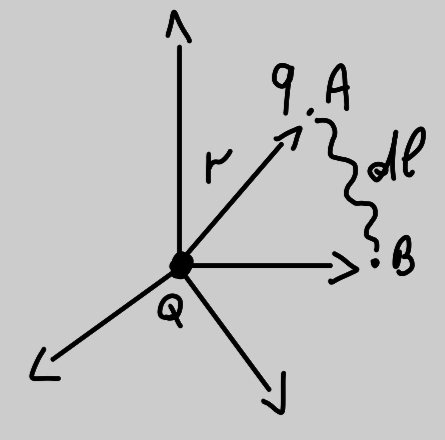
\includegraphics[width=0.5\textwidth]{energia_elettrostatica_1.jpg}
\end{center}
\begin{itemize}
    \item Q è la particella che genera il campo elettrico
    \item q invece è la particella che si sposta da A a B
    \item $dL = \vec{F}\vec{dl}$
    \item $dL = \frac{qQ}{4\pi\epsilon_0r^2}\hat{r}\vec{dl}$
\end{itemize}
$\hat{r}\vec{dl}$ non è nient'altro che la proiezione di $r$ su $dl$ ovvero $dr$
\newline Il lavoro da A a B invece equivale all'integrale
\begin{quote}
    \begin{math}
        L_{AB} = \int^B_A dL = \frac{qQ}{4\pi\epsilon_0} \int^B_A \frac{\hat{r}\vec{dl}}{r^2} = \int^{r_B}_{r_A} \frac{dr}{r^2} 4
        = -\frac{1}{r}|^{r_B}_{r_A}
    \end{math}
    che è uguale a 
    \begin{math}
        \frac{qQ}{4\pi\epsilon_0}(\frac{1}{r_A}-\frac{1}{r_B}) = -\Delta U\\
        \newline U_{carica q} = \frac{qQ}{4\pi\epsilon_0r}+c
    \end{math}
\end{quote}
L'unità di misura dell'energia potenziale è il Joule [J]
\newline $U_\infty = 0$ perché non ci sono cariche
\newline $U = \frac{qQ}{4\pi\epsilon_0r} = -(U_\infty-U_r) = -\Delta U$

\section{Campo potenziale elettrostatico}

\begin{description}
    \item[N.B.:] le cariche sono statiche
    \item[Definizione:] $\Delta_{AB}V=\frac{\Delta U_{AB}}{q}$ 
\end{description}

Il lavoro del campo, lavoro del potenziale:
\begin{center}
    \item $L=-q\Delta V$
\end{center}

L'unità di misura del potenziale è il Volt [V].
Quindi

\begin{center}

    $\Delta U_{energia} = -\int_A^B \vec{F}\vec{dl} \Rightarrow 
\Delta V=V_B-V_A=-\int_A^B\vec{E}\vec{dl}$

\end{center}
Formula per il calcolo del potenziale:
\[
\begin{cases}
V(r_0) = V_0 = 0 & \mbox{solo in alcuni casi} \\
V(r) = -\int_{r_0}^{r} \vec{E} \vec{dl} \\
\end{cases}
\]

Che cammino scelgo per calcolare $E$? Quello più comodo. Ogni carica genera potenziale e un proprio campo.

\begin{center}
	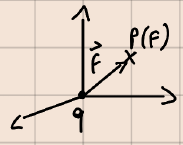
\includegraphics[width=0.5\textwidth]{gr_part.png}
\end{center}      

\[
\begin{split}
	\vec{E} (r) &= \frac{q}{4\pi \epsilon_0 r^2} \hat{r} \\
	&V(r) - V_0 = -\int_{r_0}^{r} \underbrace{\frac{q}{4\pi \epsilon_0 r^2} }_{\vec{E}(r)} \overbrace{\hat{r} \vec{dl}}^{dr} \\
	&-\frac{q}{4\pi \epsilon_0} \int_{r_0}^{r} \overbrace{\frac{1}{r^2}dr}^{=-\frac{1}{r}} \\
	&\frac{q}{4\pi \epsilon_0}[\frac{1}{r} - \frac{1}{r_0}] \\
\end{split}  
\]      

Posso porre $V_0 = 0$ con 

\[
\begin{split}
r_0 &= \infty \\
&V(r) - \underbrace{V_{\infty}}_0 = -\int{\infty}{r} \frac{q}{4\pi \epsilon_0 r^2} = \frac{q}{\pi \epsilon_0 r} \\
&V(r)_q = \underbrace{\frac{q}{4\pi \epsilon_0 r}}_{formula effettiva} [v] con V_{\infty} = 0 \\
\end{split}
\]

$V_{\infty} = 0$ è possibile solo se a $\infty$ non ci sono cariche, ciò è possibile solamente in un sistema finito.  

\paragraph{Cosa succede con N cariche discrete?}

\begin{center}
	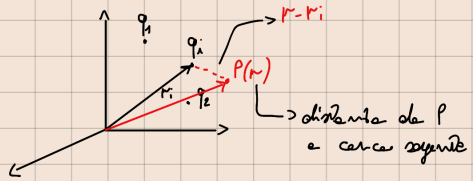
\includegraphics[width=0.5\textwidth]{discrete.png}
\end{center} 

\[
\begin{split}
\vec{E_i}(r) &= \frac{q_i}{4\pi \epsilon_0(r - r_i)^2} \hat{r - r_i} \\
&E_{TOT} = \sum E_i \\
\end{split}
\]

Per il principio di sovrapposizione si possono sommare i campi.

\[
V_{TOT}(r) = \sum_i \frac{q_i}{4\pi \epsilon_0 |r - r_i|}
\]

In una distribuzione continua \[\sum \rightarrow \int\] quindi:
\begin{center}
	\[V(r) = \frac{1}{4\pi \epsilon_0} \int\frac{dq}{r-r'}\]
\end{center}

Che può essere calcolato sullo spazio, il volume o linearmente.

\section{Linee di campo}

Sono linee tangenti al campo in ogni punto, continue ed escono dalle cariche positive mentre entrano da quelle negative.

\begin{center}
	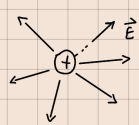
\includegraphics[width=0.5\textwidth]{left.png}
	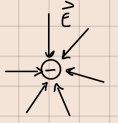
\includegraphics[width=0.5\textwidth]{right.png}
\end{center}

\section{Superfici equipotenziali(superfici in cui V è costante)}
	
\begin{center}
	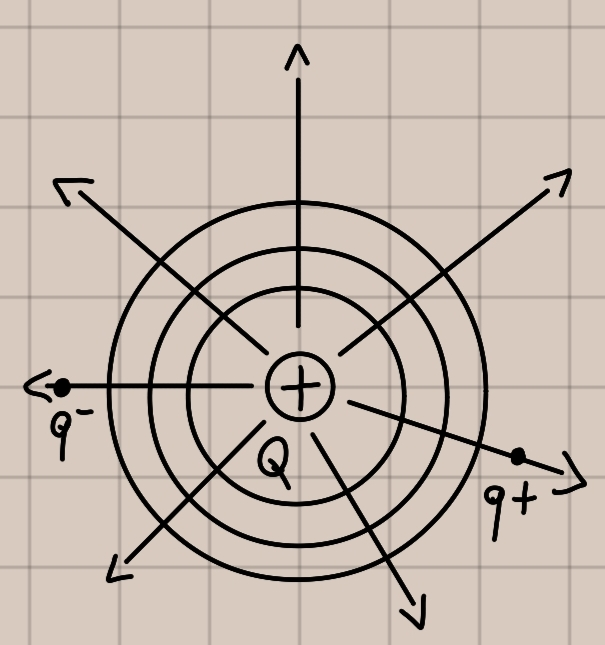
\includegraphics[width=1\textwidth]{equi.jpg}
\end{center}

La carica che genere il campo è circondata da sfere equipotenziali, la carica positiva si sposterebbe fino a \[\infty\] mentre la carica negativa verrebbe attratta fino a scontrarsi con quella che genera il campo.

\[\vec{E}(r) = \frac{\vec{F}}{q} = \frac{Q}{4\pi \epsilon_0 r^2}\hat{r}\]

Si calcoli il lavoro

\[dL = -qdV\] se \[dV = 0\] allora \[dL\] è nullo, implica che la forza generata è perpendicolare alla superficie equipotenziale.

\begin{description}
	\item[N.B.:] il lavoro è negativo quando ci si sposta nella direzione opposta alla forza
\end{description}

Una particella lasciata libera e non fissa nello spazio avrebbe sempre lavoro positivo perché seguirebbe la forza a cui è sottoposta senza farne resistenza.

\begin{description}
	\item[Campo elettrostatico] è conservativo, ovvero esiste una \[V\] t.c. il \[L_q = -\Delta V\]
\end{description}

Il lavoro svolto in un percorso chiuso sarà sempre equivalente a zero, la \textbf{Prima equazione di Maxwell} afferma che:
\begin{itemize}
	\item \[\oint_{\gamma} \vec{E}\vec{dl} = 0 \]
\end{itemize}

\section{Teorema di Gauss}

Viene usato per calcolare \[\vec{E}(r)\] Prendiamo una carica puntiforme $q$. Il campo è costante mantenendo fissa una certa distanza, di conseguenza moltiplicando \[\vec{E}\textrm{ per la superficie della sfera}\] si otterrà una costante.

\begin{description}
	\item[N.B.:] un angolo solido è \[d\Omega = \frac{dS_{sferica}}{r^2} = \frac{\hat{r}\hat{n}dS}{r^2}\]
\end{description}

\paragraph{Flusso del campo $\vec{E}$}

\begin{center}
	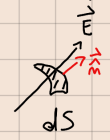
\includegraphics[width=0.5\textwidth]{flusso.png}
\end{center}
\begin{description}
	\item[Flusso elementare] $d\Phi = \vec{E}\vec{dS}$
\end{description}
Dove $\vec{dS} = dS\hat{n}$, il flusso attraverso una superficie equivale a \[\Phi(E) = \int_{sup} \vec{E}\overbrace{\hat{n}dS}^{\vec{dS}}\] che ha come unità di misura \[[\Phi] = [E][superficie] = \frac{V}{m}m^2 = Vm\]
Avremo inoltre che il flusso sarà:
\begin{itemize}
	\item $> 0$ quando il flusso sarà orientato con la normale di $\hat{n}$
	\item $= 0$ quando il flusso sarà perpendicolare alla normale
	\item $< 0$ quando il flusso sarà opposto alla direzione della normale
\end{itemize}

La \textbf{Seconda equazione di Maxwell} afferma che: \[\Phi(\vec{E}) = \oint_{\gamma}\vec{E}\vec{dS} = \frac{Q_{TOT}}{\epsilon_0}\]
Prendendo in considerazione una carica $q$ all'interno di una superficie e concentrandoci solo su una parte della superficie, il flusso generato dalla carica sarà 
\[
\begin{split}
	d\Phi &= \vec{E}\vec{dS}= \\
	&\frac{q}{4\pi\epsilon_0r^2}\hat{r}\hat{n}dS \\
	&\text{notare che}
	\frac{q}{4\pi \epsilon_0}\overbrace{\frac{\hat{r}\hat{n}dS}{r^2}}^{d\Omega} \\
	&\text{di conseguenza} 
	\frac{q}{4\pi \epsilon_0}d\Omega \\
\end{split}
\]
Quindi
\[
\begin{split}
\Phi &= \oint_{\gamma} d\Phi = \\
&\frac{q}{4\pi \epsilon_0}\int_{\gamma}d\Omega = \frac{q}{\epsilon_0}
\end{split}
\]
Aggiungendo altre cariche, il flusso di tutte sarà la somma dei flussi.
\paragraph{Perché le cariche esterne non influenzano?}
Perché il loro flusso è nullo essendo che entrano ed escono dalla superficie.

\chapter{Elettrostatica nei conduttori}
La sorgente del campo $E$ è una carica ${Q}$, il campo generato 
agisce sulle cariche e queste lo percepiscono, a loro volta ogni 
carica genererà un campo che verrà percepito dalle altre cariche.

La materia neutra affetta da un campo reagirà in due possibili modi:
\begin{itemize}
    \item le cariche libere si metteranno in moto;
    \item i materiali dielettrici vincoleranno le cariche.
\end{itemize}

\section{Proprietà di un conduttore in equilibrio}
\begin{SCfigure}[50][h!]
    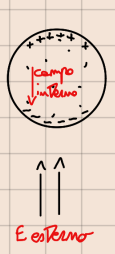
\includegraphics[width=0.3\textwidth]{conduttore.png}
    \caption{Conduttore in equilibrio}
\end{SCfigure}

La  cariche di un conduttore affetto da un campo esterno si 
sposteranno in base alla forza generata dal campo. Con questa separazione
di cariche si accende un campo interno al conduttore, indotto appunto da quello esterno.
Le cariche si sposteranno a fino a quando il campo interno non sarà nullo.

\begin{enumerate}
    \item Il campo interno di un conduttore in equilibrio è $0$, in caso contrario le particelle sarebbero ancora in movimento\[{E_{interno}} = {E_{indotto}} + {E_{esterno}} = 0\]
    \item Il potenziale nel volume del conduttore sarà costante a quello della superficie \[V = \textrm{costante}\]
    \item Se il campo fosse nullo per il teorema di Gauss la carica interna in un conduttore è $0$ \[Q_{interna} = 0\]ha solo carica superficiale \[Q_{superficiale} = \int_{superficie} \sigma dS\]
    \item Il campo della superficie dei conduttori è noto \[\vec{E}_{superficie} = \frac{\sigma}{\epsilon_0}\hat{n}\] è un campo normale alla sua superficie.
\end{enumerate}

\section{Cavità in un conduttore}

\begin{SCfigure}[50][h!]
    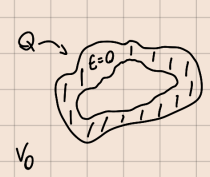
\includegraphics[width=0.5\textwidth]{conduttore_cavo.png}
    \caption[]{Conduttore cavo, con campo $E_{interno} = 0$ e potenziale $V_0$ costante}
\end{SCfigure}

Le eventuali cariche si distribuiranno solo sulla superficie del conduttore e in particolar modo la superficie della cavità interna è sempre scarica.
Quindi:

\begin{enumerate}
    \item $\sigma_{\textrm{cavità}} = 0$
    \item $\vec{E}_{\textrm{cavità}} = 0$
\end{enumerate}

\textbf{Dimostrazione:}

\begin{enumerate}
    \item Posizionando una superficie di Gauss all'interno del conduttore, abbiamo che il flusso del nostro campo sarà uguale all carica interna della superficie $S_0$ \[ \oint_S \vec{E}\vec{dS} = \frac{Q_{int}}{\epsilon_0}\] ma essendo il campo 
    di cui calcolo il flusso, il campo interno,  nullo allora la carica interna totale sarà uguale a zero \[Q_{\textrm{int totale}} = 0\] la superficie è arbitraria, quindi la posso stringere fino alla superficie della cavità, dimostrando che 
    la carica \textbf{totale} sulla superficie della cavità è nulla, \textbf{N.B.}: questo non implica che la superficie della cavità sia scarica.
    \item La carica è identicamente nulla, supponiamo che la carica totale sia nulla, ma che ci sia una separazione di carica sulla superficie della cavità, per l'elettrostatica ci sarebbe l'accensione di un campo 
    indotto dalla separazione di cariche, ricordando che la circuitazione del campo in qualsiasi cammino $\Gamma$ chiuso è sempre nulla \[ \oint_\Gamma Edl = 0 \] allora in una situazione simile io potrei sempre prendere una circuitazione $\Gamma$ posta 
    in parte all'interno del conduttore e in parte all'interno della cavità, una circuitazione simile viene calcolata come la somma degli integrali \[ \int_{\Gamma_{\textrm{conduttore}}} + \int_{\Gamma_{\textrm{cavità}}} \] la parte interna al conduttore sarà nulla 
    in quanto il campo elettrico all'interno di un conduttore è appunto nullo, quindi avrei per assurdo che la circuitazione è $\neq$ da zero, questo non è possibile che non ci troviamo in equilibrio elettrostatico e andrebbe contro l'ipotesi di partenza.
\end{enumerate}

Questo dimostra che la separazione di cariche non esiste e che la carica all'interno della cavità è identicamente nulla, questo significa a sua volte 
che non può esserci distribuzione di carica sulla superficie interna. Anche se caricassi il conduttore con una carica esterna la situazione della cavità non cambierà.
Le leggi di Maxwell richiedono che qualunque sia la situazione 
delle cariche esterne dello spazio esterno il conduttore 
andrà in equilibrio elettrostatico distrubuendo le cariche 
sulla superficie esterna.

\section{Schermo elettrostatico}

Dal punto di vista generale abbiamo un conduttore cavo, possiamo
avere delle cariche libere esterne e/o depositate sul conduttore.
In particolare nessuna situazione esterna non può influenzare 
la situazione interna, la cavità agirà da \textbf{schermo
elettrostatico}, ovvero la differenza di potenziale 
tra esterno e cavità rimarrà costante. 

\[V_{esterno} - V_{interno} = \textrm{costante}\]
Il potenziale della cavità cambierà in conseguenza all'
esterno, se non fosse così avrei modo dall'interno di 
sapere cosa succede all'esterno. Il campo elettrico nullo
fa da barriera tra esterno e interno. Quindi se dalla cavità
non ho modo di avere informazioni sull'esterno, viceversa
sarà possibile?

Ipotizziamo di inserire all'interno della cavità un altro conduttore
carico, ovviamente questo conduttore sarà in equilibrio 
e avrà un suo potenzale. Si potrà sempre posizionare 
una superficie di Gauss sul bordo della cavità, il 
flusso attraverso questa superficie deve essere ovviamente la 
carica interna che come visto sopra sarà nulla. Il conduttore
per essere in equilibrio indurrà la formazione di una 
carica uguale e opposta posizionata sulla superficie della
cavità.

\begin{center}
    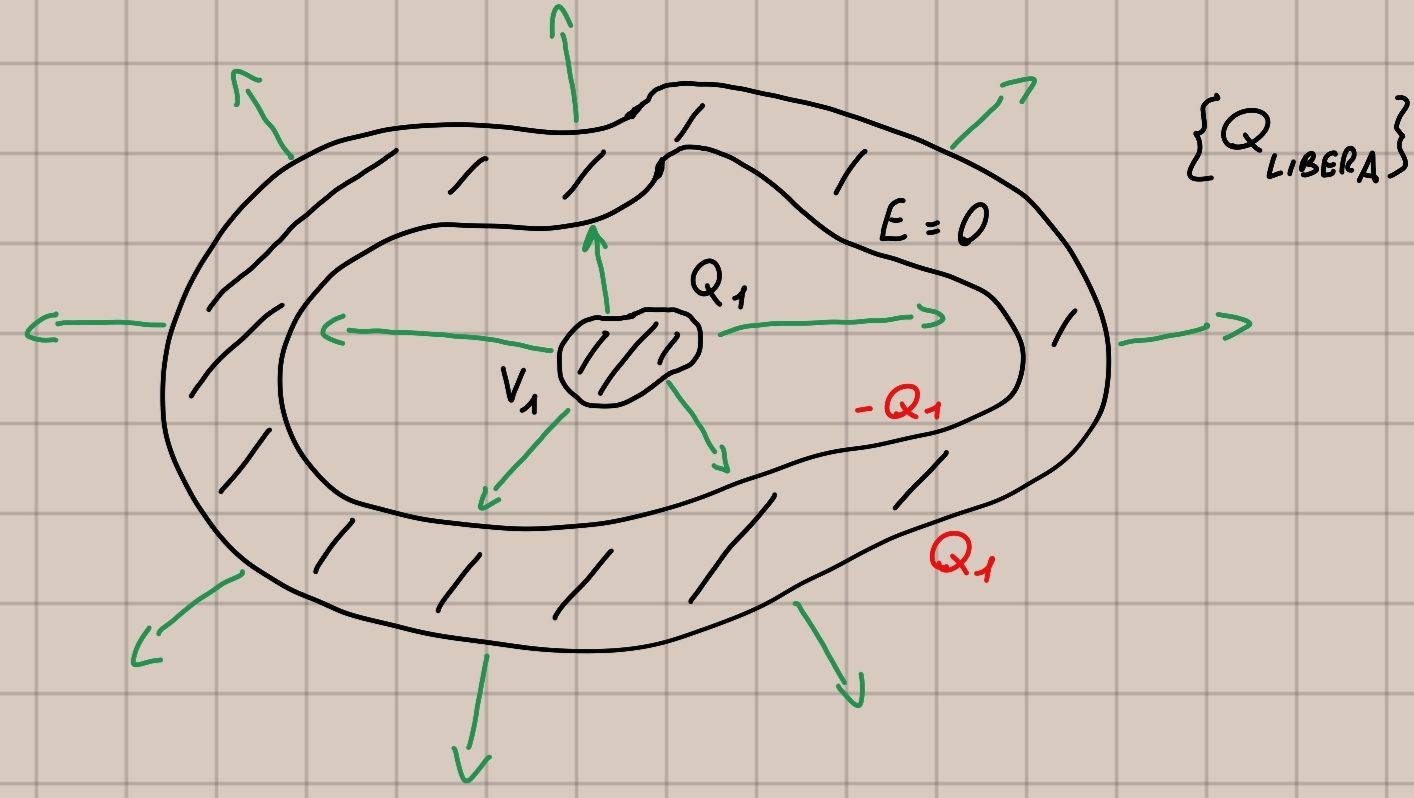
\includegraphics[width=0.5\textwidth]{conduttore_inception.jpg}
\end{center}

Poiché il conduttore esterno era inzialmente scarico, 
per la conservazione della carica dovrà comparire
una quantità di carica $-Q_1$ sulla superficie. Apparirà 
solo sull'esterno poichè all'interno deve esserci 
campo elettrico nullo. Quindi abbiamo che una carica 
interna della cavità induce una carica esterna sul conduttore.
Si potrà osservare un potenziale esterno dovuto alla 
carica $Q_1$, all'interno della cavità avremo un campo 
E $\neq$ da zero. Ricordiamo che la differenza di potenziale 
tra la regione esterna e quella interna sarà sempre 
costante.

Supponendo di aggiungere delle cariche esterne, causeranno
un cambio di potenziale, in particolare una separazione 
di cariche sulla superficie esterna. 

\begin{itemize}
    \item Cambierà qualcosa all'interno?
    \item Quanto vale la carica della cavità? 
\end{itemize}

La carica sulla superficie della cavità sarà sempre l'opposto
della carica sul conduttore interno, che ovviamente non 
potrà essere cambiata da ciò che succede all'esterno. La
cavità è uno schermo elettrostatico, questo varrà 
anche in presenza di più conduttori all'interno della 
cavità.

\section{Capacità elettrostatica}
\subsection{Conduttore isolato}

Prendiamo un conduttore isolato caricato con una carica Q,
come visto prima si porterà a un potenziale costante 
V, si definisce \textbf{capacità elettrostatica} \[ C
\frac{Q}{V} \] l'unità di misura della capacità [C] è il 
Farad (F), il significato fisico è che la carica e il 
potenziale sono proporzionali. La capacità dipende solo dalla
geometria del conduttore e in cosa è contenuto, nel nostro caso 
il vuoto.

\begin{center}
    \includegraphics[width=0.5\textwidth]{capacità_sfera.jpg}
\end{center}

Da un punto di vista pratico, prendiamo un conduttore isolato 
sferico di raggio R, depositando una carica sulla sua
superficie si genererà un campo, con un corrispondente potenziale 
nello spazio, il campo dato da \[ E = \frac{Q}{4\pi \epsilon_0 r^2} \textrm{ per r esterno} \] 
mentre il potenziale è \[ V = \frac{Q}{4\pi \epsilon_0 r} \textrm{ per r esterno} \]
Per un eventuale r interno il campo è nullo e il potenziale ovviamente 
è costante. Il potenziale sulla superficie della sfera 
per $r = R$, quindi  \[ C = \frac{Q}{V_{\textrm{superficiale r=R}}} = 4\pi \epsilon_0 R \]
è la capacità di un conduttore sferico isolato. Per ottenere
la capacità di un 1 Farad occorrerà una sfera di raggio
 \[ R = \frac{1}{4\pi \epsilon_0 } = 9\cdot 10^9m \] . Si tratta 
di numeri molto grandi, di conseguenza solitamente la capacità si misura in 

\begin{itemize}
    \item $pF$ ovvero $10^{-12}F$
    \item $nF$ ovvero $10^{-9}F$
    \item $\mu F$ ovvero $10^{-6}F$
\end{itemize}

\subsection{Conduttore non isolato}

Ci possono essere altri conduttori, in modo più esteso 
la terra stessa è un conduttore, il conduttore non essendo 
isolato sente effetti di induzione elettrostatica dai 
conduttori attorno. Quale potenziale si metterà nella 
definizione di capacità? Si definiranno conduttori solo 
a induzione completa.

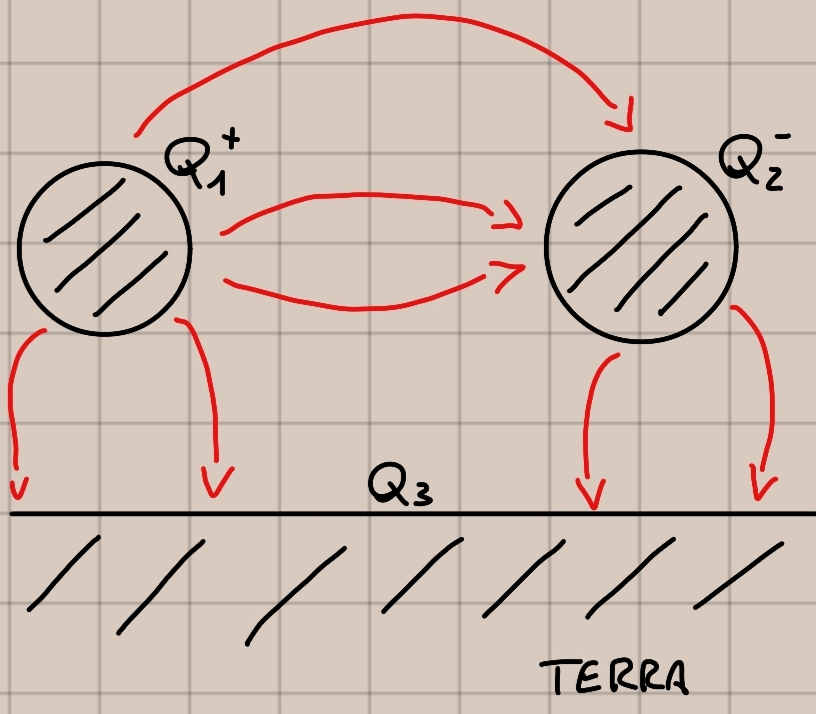
\includegraphics[width=0.5\textwidth]{cond_terra.jpg}

Si definiscono conduttori a induzione completa, due conduttori 
per cui tutte le linee di campo di uno vanno nelle 
linee di campo dell'altro. Un metodo per realizzare 
la cosa è quello di mettere uno nella cavità 
dell'altro, perché posizionando una carica sul conduttore 
interno avrò una carica indotta sulla superficie della 
cavità dell'altro. Non ci sarà alcuna dispersione delle
linee di campo. Di conseguenza la capacità si calcolerà 
come: \[ C = \frac{Q}{\Delta V} \] questa è la capacità
di due conduttori in induzione completa che si definisce 
anche \textbf{condensatore} i due conduttori si chiamano
\textbf{armature} del condensatore. 

Eventualmente le 
due armature potranno essere cilindriche, con la lunghezza 
di molto maggiore al raggio, in tal caso si potranno ignorare 
gli effetti di induzione esterna e si potrà considerarli 
in induzione completa.

Un ultimo caso sono due armature 
sottoforma di superfici, affiancate, di modo che la loro 
distanza sia molto minore della lunghezza delle superfici, 
che in maniera simile al cilindro si rirtroveranno in 
induzione completa.

\section{Collegamento di condensatori}

Collegamento in \textbf{serie}.

\begin{center}
    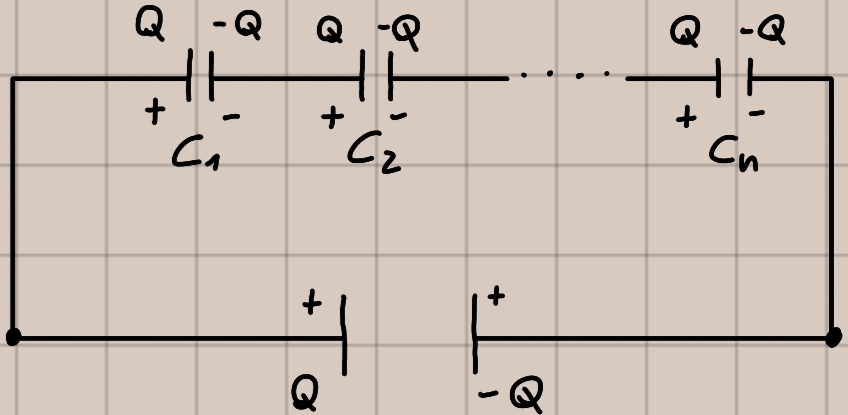
\includegraphics[width=0.5\textwidth]{coll_serie.jpg}
\end{center}
Tale collegamento ha la caratteristica che la carica 
$Q$ è sempre la stessa e che il potenziale totale è dato 
da \[ V_{TOT} = \sum_{i = 1}^n V_i \] quindi ricordando 
che la capacità equivale a \[ C_{TOT} = \frac{Q_{TOT}}{\Delta V_{TOT}} \]
avremo che 
\[
    \begin{split}
        V_{TOT} &= \Delta V_{TOT} \\
        &= \sum \frac{Q_i}{C_i} \textrm{ Q essendo costante la si porta fuori} \\
        &= Q \sum \frac{1}{C_i} \\
        &= \frac{Q_{TOT}}{C_{TOT}} \textrm{ Q totale = Q}
    \end{split}
\]
Avremo quindi che la capacità totale di un collegamento 
in serie sarà data da \[ \frac{1}{C_{TOT}} = \sum_{i = 1}^n \frac{1}{C_i} \]
Da notare che in serie la \textbf{capacità} tende a \textbf{calare} con 
l'aumentare dei condensatori.

Collegamento in \textbf{parallelo}.

\begin{center}
    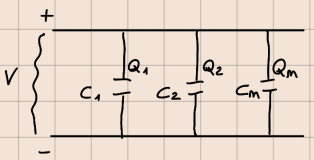
\includegraphics[width=0.5\textwidth]{coll_parall.png}
\end{center}
Nel collegamento in parallelo a rimanere costante sarà 
il potenziale. La carica $Q$ di un eventuale capacitore 
equivalente sarà la somma delle cariche dei singoli 
capacitori \[Q_{TOT} = \sum_{i = 1}^n Q_i \] ricordando 
la definizione di \textbf{capacità} avremo che \[ Q_{TOT}
\sum C_i V_i = V \sum C_i = V_{TOT} C_{TOT} \] Cosa succede 
alla capacità di un collegamento in parallelo? La carica 
aumenta, il potenziale è \textbf{costante}, quindi la 
capacità \textbf{aumenterà}.

\section{Partitore capacitivo}

Consiste nel collegamento di condensatori in serie, 
come si ripartisce il potenziale negli elementi del circuito?
Avere la stessa carica $Q$ costante significa che \[ Q = 
C_1 V_1 = C_2 V_2 = \dots = C_n V_n \] di conseguenza
\[ Q = C_{TOT} V{TOT} \] il potenziale è \textbf{inversamente 
proporzionale} alla capacità nei collegamenti in serie.
\[ V_i = \frac{Q}{C_i} = \frac{C_{TOT}}{C_i} V_{TOT} \]
Prendiamo un caso esempio con quattro condensatori con 
un interrutore aperto.
\begin{center}
    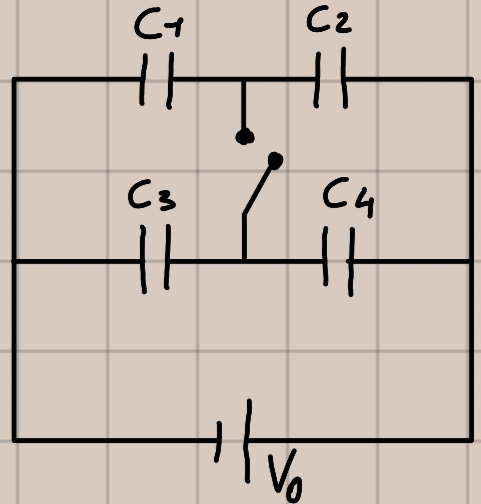
\includegraphics[width=0.5\textwidth]{int_aperto.jpg}
\end{center}
Proviamo a calcolarne la capacità totale. In questo caso
$C_1$ e $C_2$ sono collegati in serie come lo sono anche 
$C_3$ e $C_4$. Il capacitore formato da $C_1$ e $C_2$ sarà 
dato da \[ \frac{1}{C_{TOT}} = \sum \frac{1}{C_i} \] 
quindi \[ \frac{1}{C_{12}} = \frac{1}{C_1} + \frac{1}{C_2} = \frac{C_2 + C_1}{C_1C_2}\] 
oppure \[ C_{12} = \frac{C_1C_2}{C_1+C_2}\]  analogamente 
\[ C_{34} = \frac{C_3C_4}{C_3+C_4}\] i capacitori 
$C_{12}$ e $C_{34}$ sono a loro volta collegati in parallelo 
perché ai capi hanno la stessa \textbf{differenza di potenziale} ovvero $V_0$.
\begin{center}
    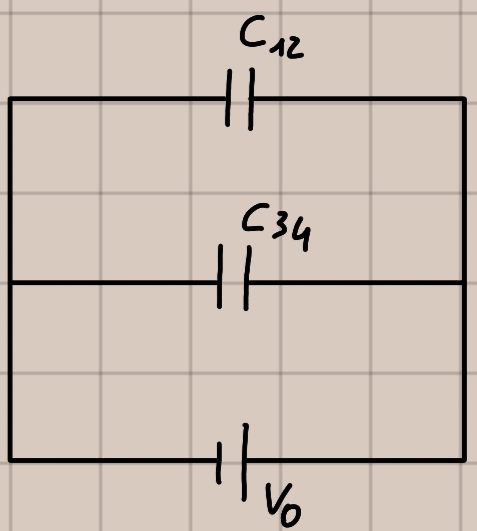
\includegraphics[width=0.5\textwidth]{coll_parall_2.jpg}
\end{center}
Il circuito equivalente sarà dato da 
\begin{center}
    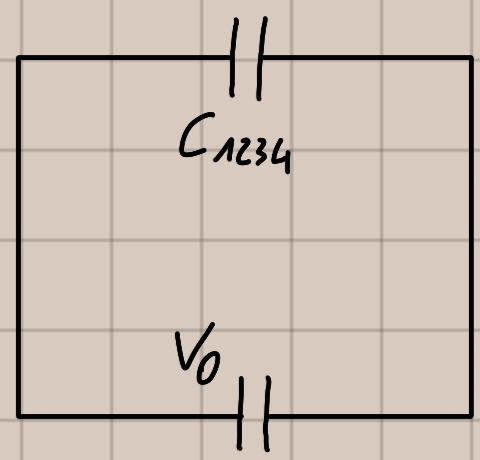
\includegraphics[width=0.5\textwidth]{coll_parall_3.jpg}
\end{center}
\[C_{1234} = C_{12} + C_{34} \] 
Se invece l'interruttore fosse chiuso 
\begin{center}
    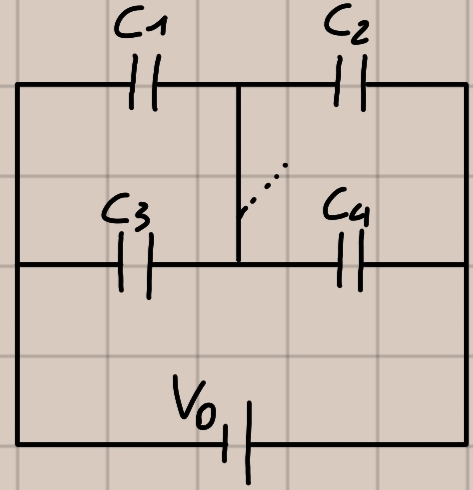
\includegraphics[width=0.5\textwidth]{int_chiuso.jpg}
\end{center}
$C_1$ e $C_3$ diventano collegati in parallelo e analogamente
$C_2$ e $C_4$ e diventa 
\begin{center}
    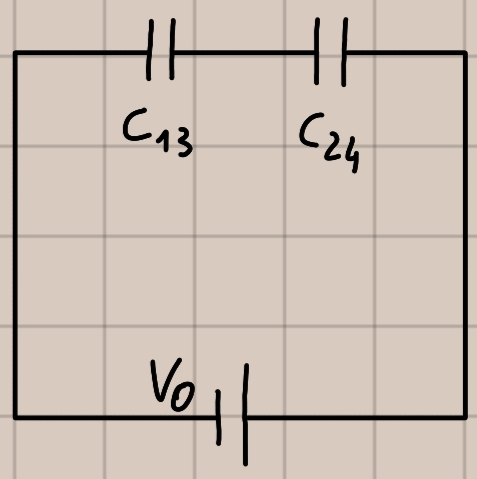
\includegraphics[width=0.5\textwidth]{int_chiuso2.jpg}
\end{center}
Essendo collegati solo a un estremo saranno collegati in serie.
La capacità totale si calcolerà similarmente a come fatto prima.

\section{Lastra conduttrice in un condensatore}

Ipotizziamo di inserire una lastra conduttrice tra le 
armature di un condensatore.
\begin{center}
    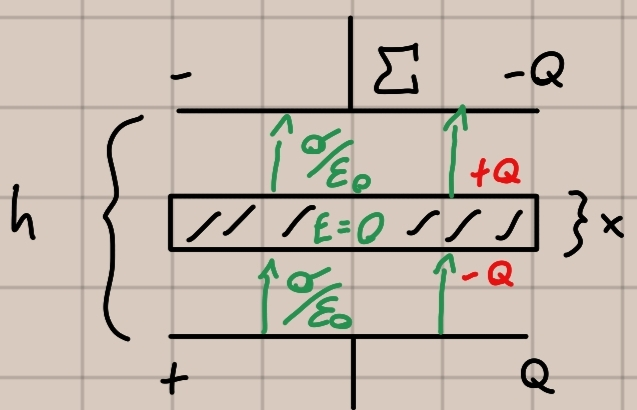
\includegraphics[width=0.5\textwidth]{lastra.jpg}
\end{center}
Ricordando che $Q$ è costante, essendo il sistema \textbf{isolato}
e $\Sigma$ equivalente all'area delle armature e che:
\[
    \begin{split}
        &E = \frac{\sigma}{\epsilon_0} \\
        &\sigma = \frac{Q}{\Sigma} \\
        &C = \frac{Q}{\Delta V} \\
        &= \frac{\sigma \Sigma}{\frac{\sigma}{\epsilon_0} h} \\
        &= \frac{\epsilon_0 \Sigma}{h} \\
    \end{split}
\]
Ricordando che \[ \Delta V = V^+ - V^- = - \int_-^+ \vec{E} \vec{dl} \Rightarrow V = Eh = \frac{\sigma}{\epsilon_0}h \] 
Il potenziale aumenterà allontando le armature perché ci vuole più 
lavoro per lo spostamento. Inserendo la lastra conduttrice
avremo un collegamento di condensatori in serie, il potenziale 
sarà minore a causa del conduttore perché avrà un campo nullo al suo interno.
Al calare del potenziale aumenterà la capacità, il potenzale
dovrà essere calcolato considerando la lasta in mezzo:
\[ V = Eh_1 + 0x + E_h2 = E(h - x) \] quindi la capacità
sarà equivalente a \[ \frac{1}{C} = \frac{h_1}{\epsilon_0 \Sigma}
+ \frac{h2}{\epsilon_0 \Sigma} = \frac{(h - x)}{\epsilon_0 \Sigma} \] 
avremo che la \textbf{capacità} effettiva con la lastra 
sarà equivalente a \[ C_{lastra} = \frac{\epsilon_0 \Sigma}{h - x} \] 

\section{Energia}

Quale lavoro bisogna compiere per caricare le armature 
di un condensatore? Quanta energia è immagazzinata nelle 
armature? Prendiamo due armature scariche e le carichiamo 
sottraendo una carica $Q$ dalla prima armatura e posizionandola
sulla seconda, ciò porterà a caricare con carica $+Q$ una 
e con carica $-Q$ l'altra. Notare che la carica totale 
rimarrà in ogni istante nulla. Successivamente il lavoro 
per traspostare una carica $q$ da una parte all'altra per 
la differenza di potenziale sarà dato da 
\[ 
    \begin{split}
        L_{\textrm{TOT ext}} &= \int_0^Q V(q) dq \\
        &= \int_0^Q \frac{q}{C} dq = \\
        &= \frac{1}{2} \frac{Q^2}{C} = U_{sistema} \\
    \end{split}
\] 
Ricordando che $C = \frac{Q}{V} \rightarrow V = \frac{q}{C}$
Questo lavoro totale esterno è l'energia immagazzinata 
nel sistema. Quindi l'energia immagazzinata in un condensatore 
è \[ U = \frac{1}{2} \frac{Q^2}{C} \] questa espressione 
si potrà esprimere in tre modi differenti: 
\begin{itemize}
    \item $U = \frac{1}{2} \frac{Q^2}{C}$
    \item $U = \frac{1}{2} CV^2$
    \item $U = \frac{1}{2} QV^2$
\end{itemize}
Si misura in Joule $[J]$. 
\begin{description}
    \item[N.B.:]  il potenziale è lineare nella carica, il potenziale ha
    sempre la carica al numeratore, sono sempre quadratiche nella carica 
    per la seconda, il potenziale va sempre con la carica, quindi 
    c'è un $Q^2$, idem per la terza, $Q\cdot V$ equivale a 
    $Q^2$. Non si scriverà \textbf{mai} $\frac{Q}{V}$.
\end{description}
\begin{center}
    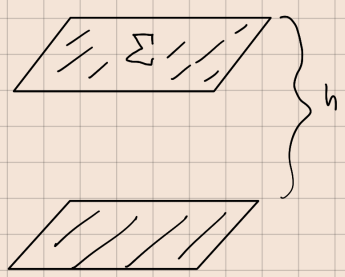
\includegraphics[width=0.5\textwidth]{lastre.png}
\end{center}
Preso un condensatore avremo 
\[
    \begin{split}
        C &= \frac{\epsilon_0 \Sigma}{h} \\
        E &= \frac{\sigma}{\epsilon_0} \\
        \sigma &= \frac{Q}{\Sigma} \\
    \end{split}
\]
sostituendo la prima e la terza all'interno di \[ U = \frac{1}{2} \frac{Q^2}{C} \]
ottengo 
\[
    \begin{split}
        U &= \frac{1}{2} \frac{Q^2}{\epsilon_0} \frac{h}{h} \\
        &= \frac{\epsilon_0}{2} E^2 \cdot \textrm{ volume} \rightarrow \Sigma h \\
    \end{split}    
\] 
Ne ricaviamo che l'energia del condensatore piano si può 
esprimere anche in questa maniera. Il volume del condensatore 
corrisponde allo spazio tra le armature, ovvero il volume 
dove il campo \textbf{non} è nullo. Quindi se in una regione 
di spazio si ha un certo campo, allora il campo 
genera una densità di energia, ovvero l'energia presente 
in un volume dello spazio, tale densità sarà:
\[ u_E = \frac{\epsilon_0 E^2}{2} \] 
unità di misura $[\frac{J}{m^3}]$ \textbf{densità di energia 
elettrostatica}.

\chapter{Elettrostatica nei dielettrici}

Sono caratterizzati dal fatto che le loro cariche sono vincolate, non sono libere di muoversi. I materiali dielettrici in presenza 
di campo esterno, mostrano la capacità di \textbf{polarizzarsi} ovvero avviene una distribuzione di carica. Un'ulteriore caratteristica 
è che i centri di carica, che normalmente nell'atomo neutro sono coincidenti, in presenza di un campo elettrico \textbf{esterno},
i costituenti carichi dell'atomo presenteranno uno spostamento dei centri di simmetria, la forza sarà data da $\vec{F} = q \vec{E}$.

Il \textbf{dipolo elettrico} è un oggetto costituito da due cariche uguali ma di segno opposto separate da una distanza rigida 
$d$ e l'orientamente sarà dalla negativa alla positiva. 
\begin{description}
    \item[Momento di dipolo elettrico:] la quantità data dalla carica per la distanza e si orienta dalla carica negativa alla positiva \[ \vec{p} = q \vec{d} \] è un vettore che caratterizza il dipolo. 
\end{description}
Il \textbf{campo di polarizzazione} sarà dato da:
\[
    \vec{P}(\vec{r}) = \frac{\textrm{momento di dipolo}}{\textrm{volume}}
\] 

\section{Proprietà del dipolo elettrico}

\begin{description}
    \item[Potenziale:] preso un punto p molto distante dal dipolo, abbastanza da non vedere la struttuta interno del dipolo. Il potenziale sarà dato da \[ V(\vec{r}) = V_{q^+} + V_{q^-} = \frac{q}{4 \pi \epsilon_0}(\frac{1}{r^+} \frac{1}{r^-}) = \frac{q}{4 \pi \epsilon_0} \frac{r^- - r^+ }{r^+r^-} \] 
    essendo $r$ la distanza presa per il punto ed essendo di molto maggiore della distanza all'interno del dipolo $d$, valgono le 
    seguente approssimazioni: 
    \begin{itemize}
        \item $r^+r^- \cong r^2$
        \item $r^--r^+ \cong d\cos \theta$
    \end{itemize} 
    Dove $\theta$ è l'angolo preso tra il centro dell'eventuale sistema di assi costruito sul dipolo e la distanza $r$ oppure 
    l'angolo che si forma sempre con la distanza $r$ ma preso da una delle cariche. Di conseguenza il potenziale sarà uguale a 
    \[ 
        V(\vec{r}) = \frac{qd\cos \theta}{r^2}
    \]
    Ricorda la definizione del \textbf{momento di dipolo} lo si può riscrivere come:
    \[
        V(\vec{r}) = \frac{\vec{p} \vec{r}}{r^3} \propto \frac{1}{r^2}
    \]
    Ricordando che $\vec{p} \vec{r}$ è nullo quando sono ortogonali, quindi il raggio vettore $r$ è perpendicolare al momento di dipolo
    $p$, di conseguenza si avrà che $V = 0$
    \begin{SCfigure}[50][h!]
        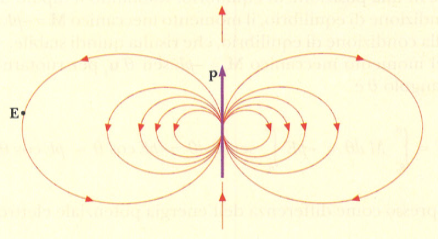
\includegraphics[width=0.5\textwidth]{dipolo.png}
        \caption[]{Linee di campo di un dipolo elettrico.}
    \end{SCfigure}
    Nel cilindro attorno all'asse centrato su $p$ non c'è modo di distinguere la fisica generata dal dipolo.
\end{description}

\section{Condensatore riempito di dielettrico}

Prendendo un condensatore piano con area $\Sigma$ e distanza $d$
\begin{center}
    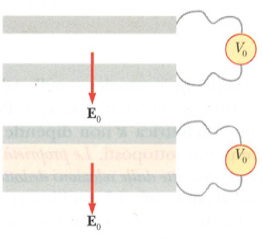
\includegraphics[width=0.5\textwidth]{condensatore_con_lastra.png}
\end{center}
Nel vuoto avremo:
\begin{itemize}
    \item $C_0 = \frac{\epsilon_0 \Sigma}{d}$ [$F$]
    \item $Q = V_0 C_0$ [$C$]
    \item $E_0 = \frac{\sigma_0}{E_0}$ [$\frac{V}{m}$]
    \item $\Delta V = E_0 d$
\end{itemize}
Isolo il sistema dal generatore, quindi la carica $Q$ sarà \textbf{costante}, inserisco un dielettrico tra le armature. Il potenziale 
sarà dal rapporto tra il potenziale nel vuoto e una costante dielettrica caratteristica del materiale, sarà di conseguenza minore del potenziale 
nel vuoto. 
\[
    V_K = \frac{V_0}{K} < V_0
\]
Se il potenziale diminuisce, la capacità di conseguenza aumenterà.
\[
    \begin{split}
        C_K &= (\frac{Q}{V}) = K C_0 \\
        C_K &= K \epsilon_0 \frac{\Sigma}{d} \\
    \end{split}
\]
$K \epsilon_0$ viene definita come \textbf{permettività} del materiale, definita normalmente come $\epsilon$. Quindi la permettività 
dielettrica del vuoto è uguale a 1 perché non c'è materiale presente.
\[
    E_K = \frac{E_0}{K} < E_0
\]
Il campo elettrico è diminuito ed è \textbf{diverso} da 0, diversamente dai conduttori. $E_K$ è il campo elettrico \textbf{totale}.
Quindi il campo indotto dai dipoli, sommato al campo precedentemente presente non dà zero. La sommma sarà equivalente a $E_K$. 
\[
    \vec{E_TOT} = E_K = \vec{E_0} + E_{\textrm{campo indotto}}
\]
Il campo indotto \textbf{non è} il campo totale.

Prendendo un condensatore elettrico con un dielettrico tra le armature, poniamo un cilindro di Gauss tra l'armatura e il 
dielettrico. Per il teorema di Gauss, il flusso passerà solo attraverso l'area del cilindro interno al dielettrico, essendo che il campo 
nella parte interna al condensatore è nullo per definizione.
\begin{center}
    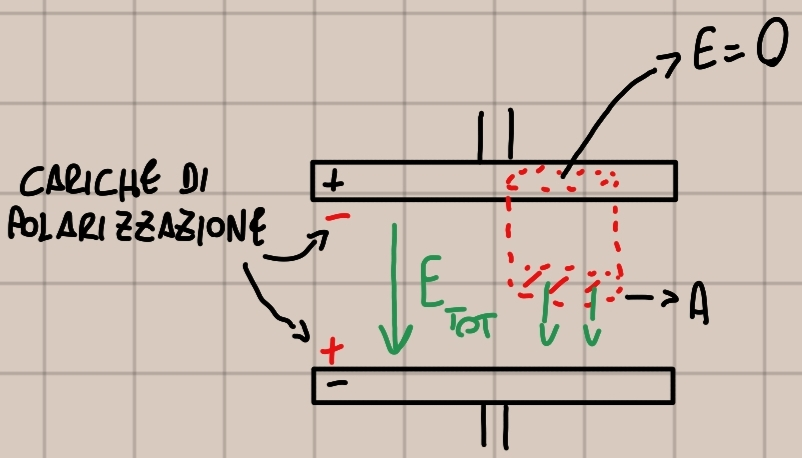
\includegraphics[width=0.5\textwidth]{cond_diel_campo.jpg}
\end{center}
Ricordando che per il teorema di Gauss, il flusso è dato da $\oint_{sup} \vec{E} \vec{dS}$ avremo che 
\[
    E_TOT A + EA = \frac{Q_{int}}{\epsilon_0}
\]
Le cariche interne a questo cilindro saranno date dalle cariche libere del conduttore più le cariche di polarizzazione indotte 
nel materiale all'accensione del campo.
\[
    \frac{Q_{libere} - Q_{pol}}{\epsilon_0} = \frac{\sigma_0}{\epsilon_0} A - \frac{\sigma_p}{\epsilon_0} A
\]
Dove:
\begin{itemize}
    \item $Q_{libere} = \sigma_0 \textrm{ Area}$
    \item $Q_p = \sigma_p \textrm{ Area}$
\end{itemize}
L'area ovviamente sparisce, quindi abbiamo ricavato che il campo nel dielettrico, ovvero $E_TOT$ sarà uguale a 
\[
    E_TOT = \frac{|\sigma_0|}{\epsilon_0} - \frac{\sigma_p}{\epsilon_0}
\]
Ricordando comunque che 
\[
    E_TOT = \frac{E_0}{K}
\]
Ricordando che $E_0 = \frac{\sigma_0}{\epsilon_0}$ e mettendo il tutto assieme possiamo ricavare che:
\[
    |\sigma_p| = |\sigma_0| \frac{K - 1}{K}
\]
Questa formula ci permetterà di calcolare le cariche di polarizzazione.

Ricordiamo che per $\sigma$ si intende il numero di carica per unità di superficie, prendendo una volume unitario di una superficie,
 che momento di dipolo avremo in un volume unitario? La polarizzazione $P$ sarà esattamente la densità di carica della superficie. 
\[
    |\vec{P}| = \sigma_p
\]
$\sigma_p$ è il modulo del campo di polarizzazione. Avremo che:
\[
    \sigma_p = \vec{P} \hat{n} [\frac{C}{m^2}]
\]

\section{Dielettrico lineare}

Un dielettrico per cui se io accendo un campo, mi si forma una polarizzazione $P$ e tale polarizzazione è parallela e 
proporzionale al campo.
\[
    \vec{P} = \epsilon_0 \chi \vec{E}
\]
Dove $\chi$ sta per la \textbf{suscettività dielettrica del materiale}. Tale suscettività è costante, il dielettrico si 
definirà \textbf{normale}, ovvero sarà lineare e omogeneo. Risulta che il campo nel dielettrico, il campo totale, l'unico campo presente 
sarà uguale a
\[
    E_K = \frac{\epsilon_0}{\underbrace{1 - \chi}_{K}}
\]

\section{Teorema di Gauss nei dielettrici}

Riprendendo l'esempio con la superficie di Gauss cilindrica, si era ottenuto che 
\[
    \oint E = \frac{\sigma_{libere}}{\epsilon_0} - \frac{\sigma_{pol}}{\epsilon_0}
\]
La carica di polarizzazione è 
\[
    \sigma_p = \vec{P} \vec{n}
\]
Si può esprimere il tutto in termini integrali di flusso 
\[
    \oint E dS = \frac{q_{libere}}{\epsilon_0} - \frac{\oint \vec{P} \vec{dS}}{\epsilon_0}
\]
Ricordando in termini generali il teorema di Gauss
\[
    \oint E dS = \frac{Q_{int}}{\epsilon_0}
\]
Il valore di $Q_{int}$ nel caso del dielettrico sarà equivalente alla carica totale tra le cariche libere e polarizzate. Non avremo più 
un campo nel vuoto, ma nel dielettrico ovviamente. Il problema della cariche polarizzate è che sono dipendenti dalle caratteristiche 
microscopiche del materiale, a noi interessa un teorema di Gauss in cui vengono usate esclusivamente le cariche libere, perché le possiamo 
controllare più facilmente (depositandole sui conduttori, attaccando potenziali,...).

La nuova definizione del teorema sarà quindi 
\[
    \begin{split}
        \oint E dS &= \frac{q_{libere}}{\epsilon_0} - \frac{\oint \vec{P} \vec{dS}}{\epsilon_0} \\
        \oint \underbrace{(\epsilon_0 \vec{E} + \vec{P})}_{*} dS &= Q_{libere} \\
    \end{split}
\]
(*) lo definisco come $\vec{D}$, è un nuovo campo e verrà definito come \textbf{induzione dielettrica}. Posso esprimere il \textbf{teorema 
di Gauss per i dielettrici} in notazione compatta come 
\[
    \oint \vec{D} \vec{dS} = Q_{\textrm{int. totali libere}}
\]
Quindi senza le cariche polerizzate. 

Il nostro scopo è sempre stato quello di calcolare il campo usando il teorema di Gauss, in presenza di materiali dielettrici non
 possiamo farlo senza pensieri perché le cariche polarizzate genereranno a loro volta un campo che andrà a sommarsi a quello totale.
 Utilizziamo Gauss per ricavare $\vec{D}$
\[
    \begin{split}
        \vec{D} &= \epsilon_0 E + P \\
        P &= \epsilon_0 \chi E \\
        \vec{D} &= \epsilon_0 K \vec{E} [\frac{C}{m^2}]\\
        \vec{E_K} &= \frac{\vec{D}}{\epsilon_0 K} \\
        P &= \epsilon_0 (K - 1) \vec{E} [\frac{C}{m^2}] \\
        \vec{P} &= \frac{K - 1}{K} D \\
    \end{split}
\] 
Trovata la polarizzazione, alla richieste del valore delle cariche su una certa superficie $s$
\[
    \sigma_p (s) = P (s)
\]

\chapter{Energia elettrostatica}

Un particella dentro l'effetto di un campo elettrico 
sentirà una forza calcolabile come \[ \vec{F} = q\vec{E} \] 
Ricordando che la forza elettrostatica del campo è 
\textbf{conservativa} possiamo ottenere che \[ L = \Delta U \] 
Ponendo $U_\infty = 0$, la possiamo riscrivere come \[ L 
= q\Delta V \] con l'energia all'infinito uguale a 0, 
l'energia del sistema sarà equivalente al lavoro \textbf{totale
contro il campo} per "costruire" il sistem.

Una distribuzione discreta di cariche q, ponendo il potenziale 
all'infinito uguale a zero ci porterà i seguenti risultati.
\begin{itemize}
    \item $L_1 = 0$ perché spostando la prima carica da 
    infinito nel sistema, non essendoci cariche presenti
    non verrà svolto del lavoro;
    \item $L_2 = (q_2 \Delta V_1) = q_2 V_1(r_2) = q_2 \frac{q_1}{4 \pi \epsilon_0 r_2}$
    \item $L_N = q_N (\Delta V_{\textrm{TOT altre cariche}} = 
    q_N (V_1(r_N)) + \dots + \underbrace{V_i(r_N)}_{(*)} + \dots + V_{N-1} (r_N))$ (*) = $\frac{q_i}{4 \pi \epsilon_0 r_N}$
\end{itemize}
Da cui si ricava che l'energia elettrostatica sarà 
equivalente a \[ U_{el} = \frac{1}{2} \sum_i^N q_i V_i = 
\frac{1}{2} \sum_{i=1}^N \sum_{j\neq i}^N q_i \frac{q_j}{4 \pi \epsilon_0 r_{ij}} \]
In distribuzione continua avremo quindi che 
\[ \begin{split}
    dU_{el} &= \frac{\overbrace{\rho(r_1)d\tau_1}^{dq_1}\overbrace{\rho(r_2)d\tau_2}^{dq_2}}{4\pi \epsilon_0 r_{12}} \\
    U_{el} &= \frac{1}{2} \int_{\textrm{volume}}\int \frac{\rho(r_1)\rho(r_2)}{4 \pi \epsilon_0 r_{12}}d\tau_1d\tau_2 \\
    &= \frac{1}{2} \int_{\textrm{volume}} \rho (r) V(r) d \tau 
\end{split}
\]

\section{Sistema di conduttori}

L'energia in un sistema con due conduttori verrà ricavata da 
\[
    \begin{split}
        U_{el} &= \frac{1}{2} \sum_{i=1}^2 Q_i V_i =  \frac{1}{2} (Q_1 V_1 + Q_2 V_2) \\
        &= \frac{1}{2} C \Delta V^2 = \frac{1}{2} \frac{Q^2}{C} = \frac{1}{2} QV \\
    \end{split}
\]

\chapter{Elettrodinamica - conduzione elettrica}

\[
    \begin{cases}
        \oint_{sup} EdS = \frac{Q_{int}}{\epsilon_0} \\
        \oint_{\Gamma} EdL = 0
    \end{cases}
\]
Sono le equazioni di Maxwell, con l'introduzione della 
variabile tempo ci ritroveremo con la prima che continuerà 
a valere, mentre la seconda no, siccome in elettrodinamica
il campo elettrico \textbf{non} è conservativo.

\section{Corrente elettrica - Forza elettromotrice}

Prendiamo due conduttori collegati tra loro da un terzo conduttore,
uno con potenziale maggiore dell'altro. Le cariche in moto 
verranno definite come \textbf{corrente elettrica} o 
\textbf{transiente} di cariche in moto.
\begin{center}
    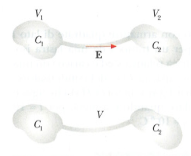
\includegraphics[width=0.5\textwidth]{conduttori_corrente.png}
\end{center}
Prendendo un generatore come in figura
\begin{center}
    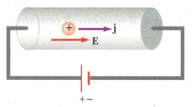
\includegraphics[width=0.5\textwidth]{gener.png}
\end{center}
noteremo che le cariche si spostano contro la direzione del 
campo, avverrà un lavoro esterno contro il campo 
elettrostatico. Tale \textbf{forza elettromotrice}
f.e.m. la si calcolerà come
\[
    \varepsilon = + \int_A^B (\frac{F}{q}) dL = V_B^+ - V_A^-
\]
Dove AB sono i capi del generatore. Ricordando che 
il elettrostatico di un circuito chiuso è nullo avremo quindi 
che
\[
    \varepsilon = \oint E dL
\]
Che ovviamente si misura in Volt [V].

\section{Intensità di corrente}

La quantità di carica che passa in un'unità di tempo 
attraverso una certa superficie.
\[
    i = \frac{dq}{dt}
\]
Unità di misura è l'ampére [A]

\section{Densità di corrente}

Quantità di caricare che attraversa una superficie
unitaria messa diagonalmente al flusso di cariche.
\begin{center}
    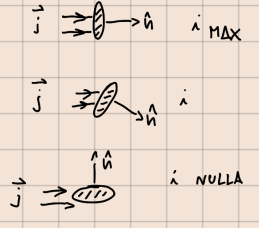
\includegraphics[width=0.5\textwidth]{dens_corr.png}
\end{center}
Avremo che 
\[
    i = \int_{sup} \vec{j} \vec{dS}
\]
Che si misurerà come [$\frac{A}{m^2}$]. Da un punto di 
vista microscopico avremo che 
\[
    i = Nq_evdSn
\]
Dove
\begin{itemize}
    \item $N$ sta per il numero di elettroni per unità di volume 
    \item $q_ev$ moltiplicato per $N$ corrisponde a $\vec{j}$
    \item $n$ invece corrisponde alla normale
\end{itemize}
\textbf{N.B.:} $j$ è una costante.

\section{Corrente stazionaria}

Nella sezione del conduttore di interesse avremo che l'
intensità di corrente sarà \textbf{costante}.
\begin{center}
    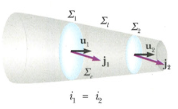
\includegraphics[width=0.5\textwidth]{corr_staz.png}
\end{center}

\section{Legge di Ohm}

\[
    V = Ri
\]
$R$, sta per \textbf{resistenza} dipende dal materiale
 e dalla sua geometria, si misura in [$\Omega$] Ohm.
\[
    R = \rho \frac{l}{s}
\]
l lunghezza del conduttore, s sezione.
\begin{center}
    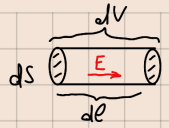
\includegraphics[width=0.5\textwidth]{ohm.png}
\end{center}
Da questa immagine possiamo ricavare che 
\[
    dV = Rdi \begin{cases}
        di = jdS \\
        dV = Edl
    \end{cases}
\]
quindi 
\[
    \vec{E} = \rho \vec{j}
\]
e 
\[
    \vec{j} = \sigma \vec{E}
\]
dove $\sigma$ è la \textbf{conducibilità elettrica}
inversamente proporzianle alla resistività
\[
    \rho = \frac{1}{\sigma}
\]

\section{Potenza elettrica - Effetto Joule}

Ricordando che la potenza è equivalente a 
\[
    P = \frac{dL}{dt}
\]
e che 
\[
    dL = Vdq
\]
dove per $L$ si intende quella del generatore, ricaveremo 
che 
\[
    P = Vi
\]
che si misura in Watt [W], la potenza elettrica erogata
dal generatore. \textbf{SE} se vale Ohm, allora 
\[
    P = Ri^2 = \frac{V^2}{R}
\]
L'effetto Joule produce calore dalla potenza dissipata 
dal resistore.

\section{Bilancio energetico}

Ricordando che in presenza di una resistenza avremo 
che la differenza di potenziale sarà equivalente a 
\[ V = Ri \] per il calcolo della differenza di potenziale.
\textbf{N.B.:} il potenziale per noi sarà sempre positivo.
La corrente scorre sempre dal (+) al (-), caduta di 
potenziale.

Per far circolare la corrente in un circuito sarà necessario 
mettere un generatore, che ripristina il salto 
di potenziale. Un generatore eroga una potenza equivalente 
a \[ P_{erogata} = \mathcal{E} i \] questa viene usata nel circuito da 
tutti i dispositivi collegati. Il resistore in particolare 
dissipa sempre una potenza \[ P_{dissipata} = (Vi) = Ri^2 \] è \textbf{sempre} 
maggiore di zero. Il bilancio energetico sarà sempre 
la potenza erogata uguale alla potenza dissipata. Se devo 
calcolare il lavoro [J] nel tempo, partendo dalla definizione 
di potenza [W] \[ P = \frac{dL}{dt} \] dovrà integrare 
la potenza nel tempo \[ L = \int Pdt \] per tutta 
la durata di tempo in cui avrò intensità di corrente 
diversa da zero. Il bilancio dei lavori darà \[ \mathcal{E}i \Delta t = Ri^2 \Delta t \] 

Partendo dalla figura
\begin{center}
    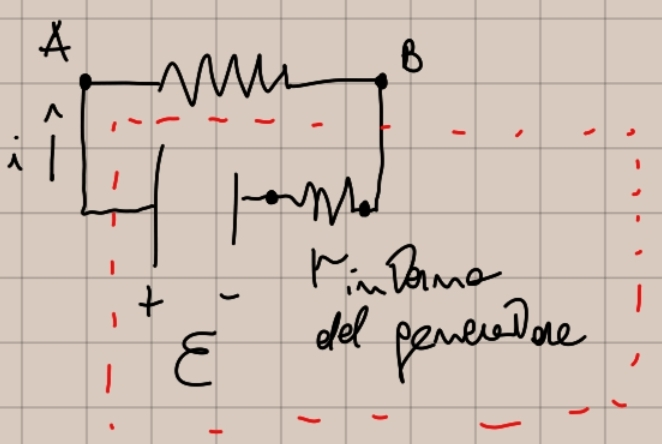
\includegraphics[width=0.5\textwidth]{circ_res.jpg}
\end{center}
Il verso della corrente dipende dai morsetti, mentre il 
segno dipende dal verso che associo al circuito. La forza 
elettromotrice del generatore sarà spesa per generare 
il salto di potenziale, che sarà la somma totale dei potenziale 
persi nel circuito. \[ \mathcal{E} = Ri + ri \] la differenza 
di potenziale ai capi A e B sommata alla differenza di 
potenziale tra la resistenza del generatore. Il seguente 
grafico mostra la caduta di potenziale lungo il circuito:
\begin{center}
    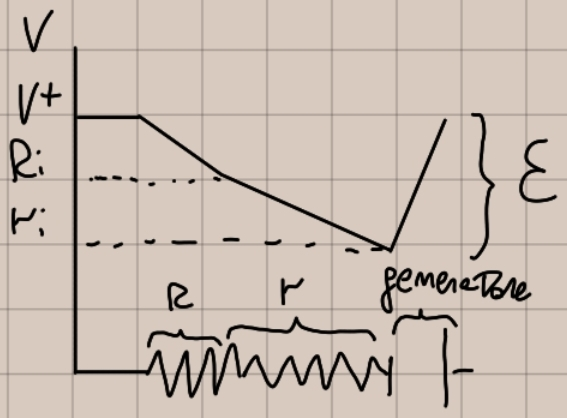
\includegraphics[width=0.5\textwidth]{graf_potenziale.jpg}
\end{center}
La differenza di potenziale sarà \[ V_A - V_B = Ri = \mathcal{E} - ri < \mathcal{E} \]
L'intensità di corrente sarà \[ i = \frac{\mathcal{E}}{R + r} \] 
mettendo tutto assieme avremo che \[ \mathcal{E} - r \frac{\mathcal{E}}{R + r}\] 
raccogliendo $R$ avremo \[ V_A - V_B = \frac{\mathcal{E}}{1 + \frac{r}{R}} \]
a circuito aperto, ovvero con $R\rightarrow \infty$ e $i\rightarrow 0$ avremo 
\[V_A - V_B = \mathcal{E}\]

\section{Bilancio energetico nel potenziale}

Il bilancio in potenziale:
\[ \mathcal{E} = Ri + ri \] che per definizione vale 
per carica unitaria. Per una carica q generica avremo 
\[ dq = idt \] avrò quindi il bilancio in energia:
\[ \mathcal{E}idt = Ri^2dt + ri^2dt \] togliendo $dt$ 
avrò il bilancio nelle potenze:
\[ \mathcal{E}i = Ri^2 + ri^2 \] 

\section{Resistori}

Possono essere in
\begin{itemize}
    \item serie, in cui le intensità di corrente sono equivalenti, mentre \[ V_i = R_i i \] 
    \item parallelo, le differenze di potenziale sono equivalenti.
\end{itemize}
\begin{figure}[h!]
    \centering
    \subfloat[][\textbf{\emph{Resistori in serie}}]
    {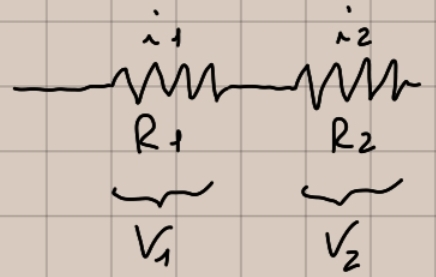
\includegraphics[width=0.3\textwidth]{res_serie.jpg}}\quad
    \subfloat[][\textbf{\emph{Resistori in parallelo}}]
    {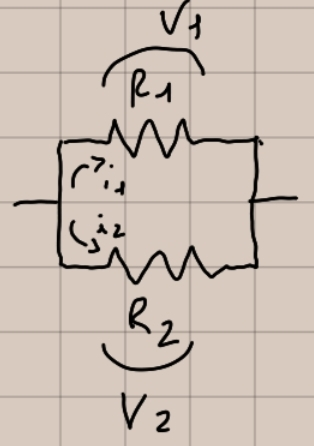
\includegraphics[width=0.3\textwidth]{res_parallello.jpg}}\\
\end{figure}
L'obiettivo è di trovare la resistenza equivalente di entrambi 
i casi.
\begin{description}
    \item[Def:] la resistenza equivalente è quella resistenza per cui se io prendo una differenza di potenziale ai capi di un collegamento, io avrò \[ V_{TOT} = R_{eq}i_{TOT} \] 
\end{description}

\subsection{Collegamento in serie}

Il potenziale da un morsetto e l'altro sarà la somma dei potenziali:
\[ V_{TOT} = \sum^N_i V_i = \sum R_i i \] la corrente è costante e quindi avremo 
\[ R_{eq} = \sum_{i = 1}^N Ri \]

\subsection{Collegamento in parallelo}

La corrente totale sarà la somma delle correnti che escono 
dai nodi, con il segno scelto convenzionalmente, ciò che 
entra deve essere uguale a ciò che esce. 
\[ i_{TOT} = \sum^N_i i_i = \sum \frac{V_i}{R_i} \] il potenziale 
in questo caso è costante, quindi avremo \[ R_{eq} = (\sum \frac{1}{R_i})^{-1} \]

\subsection{Esempio}

\begin{center}
    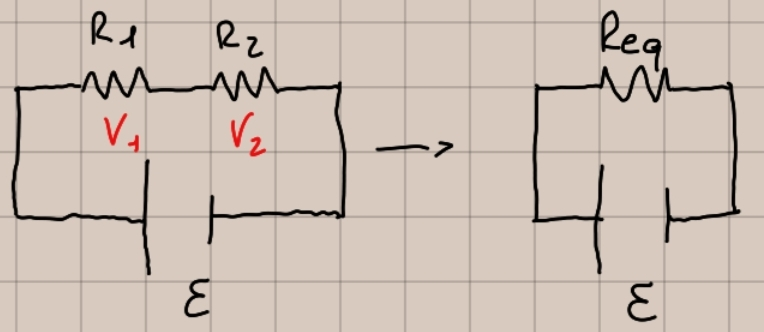
\includegraphics[width=0.5\textwidth]{es_serie.jpg}
\end{center}

\[ R_{eq} = R_1 + R_2 \] 
L'intesità di correnti che scorre su $R_1$ è equivalente a quella 
che scorre su $R_2$ \[ i = i_1 = i_2 = \frac{\mathcal{E}}{R_1 + R_2} = \frac{\mathcal{E}}{R_{eq}} \]
che si misura ovviamente in ampére [A].

La differenza di potenziale ai capi della resistenza $R_1$ sarà 
\[ V_1 = R_1i = \frac{R_1 \mathcal{E}}{R_1 + R_2} \] 
analogamente la differenza di potenziale ai capi della seconda 
resistenza sarà \[ V_2 = \frac{R_2 \mathcal{E}}{R_1 + R_2} \] 
volt [V]. I potenziali vengono ripartiti.

Ovviamente \[ V_1 + V_2 = \mathcal{E} \] 

Se invece collego in parallelo due resistori 
\begin{center}
    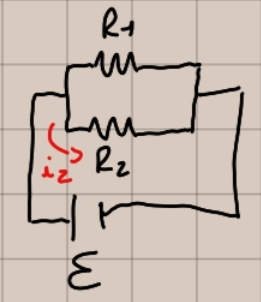
\includegraphics[width=0.5\textwidth]{es_parall.jpg}
\end{center}
\[ R_{eq} = \frac{R_1R_2}{R_1 + R_2} \] 
$V$ ai capi della resistenza è la stessa e analogamente da 
sopra, qui è la corrente che viene ripartita, siccome il potenziale
è costante.
\[ i_1 = \frac{\mathcal{E}}{R_1} = \frac{R_2}{R_1 + R_2} i \] 
analogamente
\[ i_2 = \frac{R_1}{R_1 + R_2} i \]

\subsection{Potenze}

\[ P = \sum^N P_i = \sum R_i i_i^2 = R_{eq}i^2_{TOT} \]
La potenza in serie \[ P_{serie} = (R_1 + R_2) i^2_{TOT} \] 
In parallelo \[ P_{parallelo} = R_1 i_1^2 + R_2 i_2^2 = \mathcal{E}^2 (\frac{1}{R_1} + \frac{1}{R_2}) \] 
e quindi \[ P_{parallelo} = \frac{R_1 R_2}{R_1 + R_2} i^2_{TOT} \] 
Ricapitolando, per avere la potenza totale del circuito si 
possono sommare localmente. In generale \[ P_{TOT} = R_{eq} i^2 \]

\section{Leggi di Kirchhoff}

Nelle reti lineari l'intensità di corrente è \textbf{continua} e vale la legge di Ohm.
\begin{enumerate}
    \item $\sum i_k = 0$ con il segno dato dalla convenzione del verso, in un nodo rendiamo positive le correnti uscenti e negative quelle entranti;
    \item $\sum \mathcal{E}_k = \sum R_k i_k $ con il segno delle tensioni deciso dal verso, questa è la differenza di potenziale.
\end{enumerate}
\begin{center}
    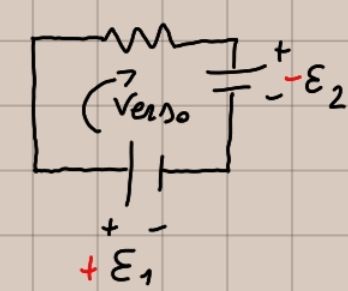
\includegraphics[width=0.5\textwidth]{segno.jpg}
\end{center}
Deciso un verso, se la corrente che risulta nella maglia è 
positiva allora sarò oraria, altrimenti antioraria. Il 
segno dei generatori è dato dal verso della maglia, se il 
generatore fornisce un lavoro per far scorrere una corrente 
nel verso della maglia il segno sara positivo. Forniscono 
una f.e.m. totale nel circuito data da \[ \mathcal{E}_1 - \mathcal{E}_2 = Ri \]
dove l'intensità non è conosciuta, ma si è deciso il segno positivo 
in quella direzione.

\section{Carica/scarica di un condensatore}

\begin{SCfigure}[50][h!]
    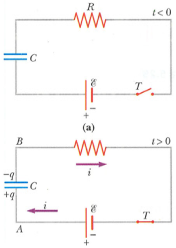
\includegraphics[width=0.5\textwidth]{scarica.png}
    \caption{Circuito di scarica del condensatore}
\end{SCfigure}
Nel circuito le cariche inizieranno a scorrere 
come in figura. La carica varierà nel tempo, la carica 
migra da un'armatura all'altra e il potenziale varia nel
tempo con la carica. Ricordiamo che la capacità la si 
calcola come \[ C = \frac{Q}{V^+ - V^-} \]
Dove $V^+ - V^- = V$.

Chiudendo l'interrutore, in un instante generico di tempo 
avremo ai capi del condensatore, avrò una differenza di potenziale 
che varia nel tempo data da \[ V(t) = \frac{Q(t)}{C} \]
L'intensità di corrente sarà data dalla carica che scorre 
\[ i = -\frac{dQ}{dt} \] Il meno dell'intensità è dato 
perché la carica Q sul condensatore diminuisce e l'intensità 
aumenta. La legge di Ohm vale, quindi \[ i(t) = \frac{V(t)}{R} \] 
in cui la differenza di potenziale è calcolata ai capi 
della resistenza.

\begin{description}
    \item[N.B.:] Se la scarica è "lenta", la differenza di potenziale ai capi 
    del resistore, in ogni momento sarà uguale a quella 
    ai capi del condensatore. 
\end{description}
Partendo quindi da queste formule otteniamo che 
\[ \frac{dQ}{dt} + \frac{Q}{RC} = 0 \] 
\[\int_{Q_0} \frac{dQ}{Q} = \int_{t_0} -\frac{dt}{RC} \] 
Avremo quindi \[ Q(t) = Q_0 e^{-\frac{t}{RC}} \] 
questa è la \textbf{legge di scarica del condensatore}. 
Derivando questa otterremo \[ i(t) = i_0 e^{-\frac{t}{RC}} \]
Quanto vale $i_0$? \[ i_0 = \frac{Q_0}{RC} = \frac{V_0}{R} \] 
Il potenziale? \[ V = V_0 e^{-\frac{t}{RC}} \]
La potenza? Dissipata dal resistore e immagazzinata 
dal condensatore, la formula sarà: \[ P = Ri^2(t) = \frac{V_0^2}{R} e^{-\frac{2t}{RC}} \] 
Quanto è l'energia totale dissipata? Quanto calore si genera? 
\[ U_{\textrm{tot dissipata}} = \int_{t_0 = 0}^{t = \infty} Pdt = \frac{V_0^2}{R} [(\frac{RC}{2})-e^{-\frac{2t}{RC}}]\mid_0^\infty = \frac{V_0^2C}{2} = U\] 
Che è esattamente l'energia immagazzinata nel condensatore.

\textbf{Analogamente} per la carica, partendo da un circuito 
scarico, mettendo un generatore che muove le cariche, queste 
andranno a caricare le armature. Partendo dalla legge di 
Ohm \[ \mathcal{E} = V_R(t) + V_C(t) \] in questa situazione 
l'intensità rispetto a prima avrà lo stesso segno delle cariche e 
la formula rimarrà la stessa \[ i = +\frac{dQ}{dt} \] 
mentre la carica \[ Q(t) = \frac{C \mathcal{E} }{Q_{finale}} (1 - e^{-\frac{t}{RC}}) \] il condensatore 
raggiungerà una carica massima data dalla forza dele generatore.
\begin{description}
    \item[N.B.:] la corrente all'istante $t_0$ è \textbf{massima} e andrà a calare man mano che si carica il condensatore.
\end{description}
\[i(t) = i_0 e^{-\frac{t}{\tau}} \] dove \[ i_0 = \frac{\mathcal{E}}{R} \] 
e \[ V(t) = \frac{Q(t)}{C} \] 

\chapter{Magnetostatica}

Si osserva che alcuni materiali (ossidi di ferro), palesano 
un'esistenza di una nuova forza, ovvero non descrivibile con le 
teoria conosciute finora. Questa forza può essere attrattiva e repulsiva
ed è localizzata ai poli (nord e sud) del materiale.
Inoltre prendendo un materiale simile, ma molto piccolo,
che chiameremo "ago magnetico", osservo che si orienta
sempre in una certa direzione, esiste un effetto magnetico
dovuto dal pianeta terra. Spezzando l'oggetto osserverò 
che non si possono isolare i poli, perché i due pezzi 
avranno dei nuovi poli. \textbf{Non} esiste il mono polo magnetico
ovvero \textbf{non esiste} la carica magnetica. Prendendo 
un filo di corrente e una lastra di materiale dielettrico cosparso di 
aghi magnetici, osserverò che gli aghi si orientano atttorno 
al filo (espierienza di Oersted) secondo delle linee concentriche, 
quindi la corrente elettrica è causa di effetti magnetici.
La sorgente del campo magnetico $\vec{B}$ è la corrente 
elettrica, che ovviamente può essere prodotto pure da una 
carica in moto.

La \textbf{forza di Lorentz} sarà data da: \[ \vec{F} = q \vec{v} x \vec{B} \] 
essendo una forza tridimensionale, il verso sarà dato 
usando la regola della mano destra.
\begin{SCfigure}[50][h!]
    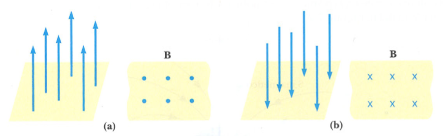
\includegraphics[width=0.8\textwidth]{frecce.png}
    \caption{Convenzione per le frecce uscenti ed entranti}
\end{SCfigure}
L'unità di misura del \textbf{campo magnetico} è il Tesla [T], 
solitamente si usa il Gauss che equivale a $10^{-4}$T.

Cosa sono le correnti? Cariche in moto, quindi mi aspetto 
un'espressione della forza che agisce sulle correnti 
partendo da quella appena trovata. Ingrandendo un filo conduttore
percorso da una certa intensità di corrente $i$, all'interno 
avrò delle cariche in moto lungo il filo $dL$, su ognuna di questa 
carica agirà una \textbf{forza di Lorentz}. Ricordando che la 
densità di corrente è data dal numero delle cariche per 
la velocità \[ \vec{j} = Nq\vec{v} \] e ricordando che 
l'intensità non è altro che \[ i = \vec{j} \vec{dS} \] 
perché è il flusso di $\vec{j}$, la somma risultante delle 
forze che agiscono su queste cariche libere, la posso esprimere 
in funzione della correnta e la lunghezza del filo. Trovo 
che su quel pezzettino di filo agisce una forza di Lorentz
complessiva, espressa come \[ dF = i\vec{dL}x\vec{B} \] 
questa è la \textbf{seconda legge di Laplace}. 

La forza magnetica compie sempre lavoro nullo, perché $dS$ 
è ortogonale a $F$. Le linee di campo di $\vec{B}$ saranno \textbf{sempre} 
chiuse perché non esiste il mono polo. Avvicinando 
una superficie chiusa, troveremo che il numero di linee 
entranti sommato a quelle uscenti sarà sempre nullo, quindi 
il flusso sarà sempre uguale a 0 \[ \Phi (\vec{B}) = 0 \] 
e sempre \[ \oint \vec{B} \vec{dS} = 0 \], si capisce 
anche che \textbf{non esiste} un potenziale magnetico.
Il flusso di $\vec{B}$ attraverso una superficie dS si misura 
in [W] Weber.

Ricapitolando non esistono sorgenti isolate, le sorgenti 
casomai sono le cariche in moto e le correnti.

Le conseguenza della \textbf{forza di Lorentz} sono tre:
\begin{enumerate}
    \item il comportamento di una spira in un campo $\vec{B}$;
    \item il moto di cariche nel campo $\vec{B}$ e $\vec{E}$;
    \item effetto Hall, un potenziale elettrico che si osserva in un sistema in cui scorre corrente elettrica e in cui si accende un campo magnetico;
\end{enumerate}

\section{Dipolo magnetico in campo esterno $\vec{B}$}

Cos'è un dipolo magnetico? Una spira elementare,
ovvero la cui geometria è così piccola da 
essere trascurabile, percorsa da corrente. Quindi a noi 
interesserà esclusamente:
\begin{itemize}
    \item l'area;
    \item il verso; 
    \item la corrente.
\end{itemize}
Definisco un parametro che racchiuda tutte queste tre cose,
ovvero il \textbf{momento di dipolo magnetico} che chiamerò 
\[ \mu = i\vec{S} \] dato dall'intensità di corrente, per l'area 
è la normale che sarà il suo verso, normale presa dal verso di i, 
tramite la regola della mano destra. Tale momento non ha 
unità di misura effettiva, sarà [$Am^2$].

Prendendo una spira percorsa da corrente i immersa in un 
campo magnetico costante. 
\begin{center}
    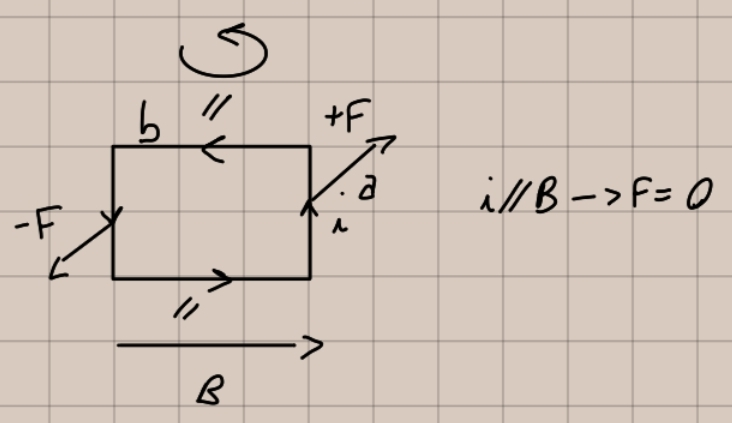
\includegraphics[width=0.5\textwidth]{spira.jpg}
\end{center}
Usando \[ \vec{F} = i\vec{dL}x\vec{B} \] e ricordando 
che un prodotto scalare è nullo quando le forze sono 
ortogonali o parallele. La risultante è nulla come 
si vede in figura, l'oggetto non trasla. Avremo un momento 
$\tau$ diverso da 0, perché l'oggetto ruota.
\[ \tau = (rxF)  = \underbrace{i\frac{ab}{S}B}_\mu \] 
da cui \[ \vec{\tau} = \vec{\mu} x \vec{B} \] 
Il momento meccanico del dipolo magnetico/spira immerso 
in campo esterno magnetico.

Quindi in presenza di un dipolo messo in qualsiasi modo 
e un campo magnetico, il dipolo si allineerà al campo, 
analogamente al dipolo elettrico. Momento di dipolo 
magnetico \[ \vec{\tau} = \vec{\mu} x \vec{B} \] 
momento di dipolo elettrico 
\[ \vec{\tau} = \vec{p} x \vec{E} \]
L'energia del dipolo è \[ U = -\vec{\mu}x\vec{B} \] 

\section{Teorema di Ampère}

Calcolando $\vec{B}$ collocato in un circuito attorno 
a un filo elettrico \[ \oint_{\Gamma} \vec{B} \vec{dL} \] 
sappiamo che $\vec{B}$ è costante ed è proporzionale a i, 
tale costante di proporzionalità o \textbf{permeabilità magnetica}
sarà \[ \mu_0 i \] dove $\mu_0$ corrisponde a $4\pi10^{-7}$ (S.I.)













\end{document}